\chapter{Used Technologies}

In this chapter the used technologies are listed. In later sections we give
some introductions to selected libraries and frameworks.


\section{Used Software}
The following software was used to develop ACE.
\begin{itemize}
 \item Java 1.4.2 (or greater)
 \item Eclipse (http://www.eclipse.org/)
 \item Ant 1.6.x (http://ant.apache.org/)
 \item Maven 2.0 Ant Tasks 2.0-beta-3 (http://maven.apache.org/)
 \item CruiseControl (http://cruisecontrol.sourceforge.net/)
 \item SubEthaEdit (http://www.codingmonkeys.de/subethaedit/)
\end{itemize}


\section{Used Frameworks and Libraries}
The dependencies of the project are specified in the Ant build file.
Here is a list of all the frameworks and libraries used directly by ACE. 
Some dependencies have additional dependencies on their own, which are 
fetched by Maven - a feature called transitive dependency handling. These
additional dependencies are not listed here.

\begin{table}[H]
 \centering
 \begin{tabular}{|l|l|}
  \hline
   \multicolumn{1}{|p{4.5in}|}{\bfseries{\textsf{Name}}} &
   \multicolumn{1}{|p{0.6in}|}{\bfseries{\textsf{Version}}} \\

  \hline
   \multicolumn{1}{|p{4.5in}|}{JDOM} &
   \multicolumn{1}{|p{0.6in}|}{1.0} \\
   \multicolumn{1}{|p{4.5in}|}{\footnotesize{\href{http://jdom.org/}{http://jdom.org/}}} &
   \multicolumn{1}{|p{0.6in}|}{} \\

  \hline
   \multicolumn{1}{|p{4.5in}|}{Commons IO} &
   \multicolumn{1}{|p{0.6in}|}{1.1} \\
   \multicolumn{1}{|p{4.5in}|}{\footnotesize{\href{http://jakarta.apache.org/commons/io/}{http://jakarta.apache.org/commons/io/}}} &
   \multicolumn{1}{|p{0.6in}|}{} \\

  \hline
   \multicolumn{1}{|p{4.5in}|}{Commons BeanUtils} &
   \multicolumn{1}{|p{0.6in}|}{1.7.0} \\
   \multicolumn{1}{|p{4.5in}|}{\footnotesize{\href{http://jakarta.apache.org/commons/beanutils/}{http://jakarta.apache.org/commons/beanutils/}}} &
   \multicolumn{1}{|p{0.6in}|}{} \\

  \hline
   \multicolumn{1}{|p{4.5in}|}{Commons Collections} &
   \multicolumn{1}{|p{0.6in}|}{3.1} \\
   \multicolumn{1}{|p{4.5in}|}{\footnotesize{\href{http://jakarta.apache.org/commons/collections/}{http://jakarta.apache.org/commons/collections/}}} &
   \multicolumn{1}{|p{0.6in}|}{} \\

  \hline
   \multicolumn{1}{|p{4.5in}|}{Commons Logging} &
   \multicolumn{1}{|p{0.6in}|}{1.0.4} \\
   \multicolumn{1}{|p{4.5in}|}{\footnotesize{\href{http://jakarta.apache.org/commons/logging/}{http://jakarta.apache.org/commons/logging/}}} &
   \multicolumn{1}{|p{0.6in}|}{} \\

  \hline
   \multicolumn{1}{|p{4.5in}|}{Glazed Lists} &
   \multicolumn{1}{|p{0.6in}|}{1.0.0} \\
   \multicolumn{1}{|p{4.5in}|}{\footnotesize{\href{http://www.publicobject.com/glazedlists/}{http://www.publicobject.com/glazedlists/}}} &
   \multicolumn{1}{|p{0.6in}|}{} \\

  \hline
   \multicolumn{1}{|p{4.5in}|}{Xerces} &
   \multicolumn{1}{|p{0.6in}|}{2.6.2} \\
   \multicolumn{1}{|p{4.5in}|}{\footnotesize{\href{http://xerces.apache.org/xerces2-j/}{http://xerces.apache.org/xerces2-j/}}} &
   \multicolumn{1}{|p{0.6in}|}{} \\

  \hline
   \multicolumn{1}{|p{4.5in}|}{Log4j} &
   \multicolumn{1}{|p{0.6in}|}{1.2.12} \\
   \multicolumn{1}{|p{4.5in}|}{\footnotesize{\href{http://logging.apache.org/log4j/docs/}{http://logging.apache.org/log4j/docs/}}} &
   \multicolumn{1}{|p{0.6in}|}{} \\

  \hline
   \multicolumn{1}{|p{4.5in}|}{JGoodies Looks} &
   \multicolumn{1}{|p{0.6in}|}{1.3.2} \\
   \multicolumn{1}{|p{4.5in}|}{\footnotesize{\href{http://www.jgoodies.com/freeware/looks/}{http://www.jgoodies.com/freeware/looks/}}} &
   \multicolumn{1}{|p{0.6in}|}{} \\

  \hline
   \multicolumn{1}{|p{4.5in}|}{Spring Framework Core} &
   \multicolumn{1}{|p{0.6in}|}{1.2.6} \\
   \multicolumn{1}{|p{4.5in}|}{\footnotesize{\href{http://www.springframework.org/}{http://www.springframework.org/}}} &
   \multicolumn{1}{|p{0.6in}|}{} \\

  \hline
   \multicolumn{1}{|p{4.5in}|}{Spring Framework Beans} &
   \multicolumn{1}{|p{0.6in}|}{1.2.6} \\
   \multicolumn{1}{|p{4.5in}|}{\footnotesize{\href{http://www.springframework.org/}{http://www.springframework.org/}}} &
   \multicolumn{1}{|p{0.6in}|}{} \\

  \hline
   \multicolumn{1}{|p{4.5in}|}{Spring Framework Context} &
   \multicolumn{1}{|p{0.6in}|}{1.2.6} \\
   \multicolumn{1}{|p{4.5in}|}{\footnotesize{\href{http://www.springframework.org/}{http://www.springframework.org/}}} &
   \multicolumn{1}{|p{0.6in}|}{} \\

  \hline
   \multicolumn{1}{|p{4.5in}|}{Spring Framework AOP} &
   \multicolumn{1}{|p{0.6in}|}{1.2.6} \\
   \multicolumn{1}{|p{4.5in}|}{\footnotesize{\href{http://www.springframework.org/}{http://www.springframework.org/}}} &
   \multicolumn{1}{|p{0.6in}|}{} \\

  \hline
   \multicolumn{1}{|p{4.5in}|}{Backport java.util.concurrent} &
   \multicolumn{1}{|p{0.6in}|}{1.1\_01} \\
   \multicolumn{1}{|p{4.5in}|}{\footnotesize{\href{http://www.mathcs.emory.edu/dcl/util/backport-util-concurrent/}{http://www.mathcs.emory.edu/dcl/util/backport-util-concurrent/}}} &
   \multicolumn{1}{|p{0.6in}|}{} \\
   
  \hline
   \multicolumn{1}{|p{4.5in}|}{concurrent} &
   \multicolumn{1}{|p{0.6in}|}{1.3.4} \\
   \multicolumn{1}{|p{4.5in}|}{\footnotesize{\href{http://gee.cs.oswego.edu/dl/classes/EDU/oswego/cs/dl/util/concurrent/intro.html}{http://gee.cs.oswego.edu/dl/classes/EDU/oswego/cs/dl/util/concurrent/intro.html}}} &
   \multicolumn{1}{|p{0.6in}|}{} \\
   
  \hline
   \multicolumn{1}{|p{4.5in}|}{DNS SD} &
   \multicolumn{1}{|p{0.6in}|}{107.1} \\
   \multicolumn{1}{|p{4.5in}|}{\footnotesize{\href{http://developer.apple.com/networking/bonjour/download}{http://developer.apple.com/networking/bonjour/download}}} &
   \multicolumn{1}{|p{0.6in}|}{} \\
   
  \hline
   \multicolumn{1}{|p{4.5in}|}{Spin} &
   \multicolumn{1}{|p{0.6in}|}{1.4} \\
   \multicolumn{1}{|p{4.5in}|}{\footnotesize{\href{http://spin.sourceforge.net/}{http://spin.sourceforge.net/}}} &
   \multicolumn{1}{|p{0.6in}|}{} \\
  \hline
 \end{tabular}
 \caption{Used frameworks and libraries}
\end{table}

\emph{JDOM} is used by the test framework only. The \emph{concurrent} library
is only used by the \emph{beepcore} implementation. 
\emph{backport-util-concurrent} is an implementation of most of the features
in \texttt{java.util.concurrent} for earlier Java versions. It is used 
because we do not use Java 1.5 and still want to use some of the advanced
features available in \texttt{java.util.concurrent}.

Further for testing we used the following frameworks:

\begin{table}[H]
 \centering
 \begin{tabular}{|l|l|}
  \hline
   \multicolumn{1}{|p{4.5in}|}{\bfseries{\textsf{Name}}} &
   \multicolumn{1}{|p{0.6in}|}{\bfseries{\textsf{Version}}} \\
  \hline
   \multicolumn{1}{|p{4.5in}|}{JUnit} &
   \multicolumn{1}{|p{0.6in}|}{3.8.1} \\
   \multicolumn{1}{|p{4.5in}|}{\footnotesize{\href{http://junit.org/}{http://junit.org/}}} &
   \multicolumn{1}{|p{0.6in}|}{} \\

  \hline
   \multicolumn{1}{|p{4.5in}|}{Easymock} &
   \multicolumn{1}{|p{0.6in}|}{1.1} \\
   \multicolumn{1}{|p{4.5in}|}{\footnotesize{\href{http://www.easymock.org/}{http://www.easymock.org/}}} &
   \multicolumn{1}{|p{0.6in}|}{} \\

  \hline
   \multicolumn{1}{|p{4.5in}|}{JMock} &
   \multicolumn{1}{|p{0.6in}|}{1.0.1} \\
   \multicolumn{1}{|p{4.5in}|}{\footnotesize{\href{http://www.jmock.org/}{http://www.jmock.org/}}} &
   \multicolumn{1}{|p{0.6in}|}{} \\

  \hline
 \end{tabular}
 \caption{Used test frameworks}
\end{table}

Additionally we used a modified version (in the subversion repository) of the
beepcore-java framework. The modifications are based on version 0.9.08. We
had to apply some patches to fix some critical bugs in the library.


\section{The Spring Framework}
\label{appendix_frameworks_spring}

The \emph{Spring Framework} is part of the movement in the \emph{Java}
community away from heavy-weigth solution based on heavy component models
back to light-weight solutions based on plain old \emph{Java} objects
(so called POJOs). It
is mainly used as a light-weight replacement for EJB containers, but it
proves to be useful outside of the Java Enterprise Edition world. The 
web page of the \emph{Spring Framework} can be found on the Spring website
(\href{http://www.springframework.org/}{http://www.springframework.org/}).

The \emph{Spring Framework} contains lots of functionality, which is grouped
into modules shown in the diagram below.

\begin{figure}[H]
 \centering
 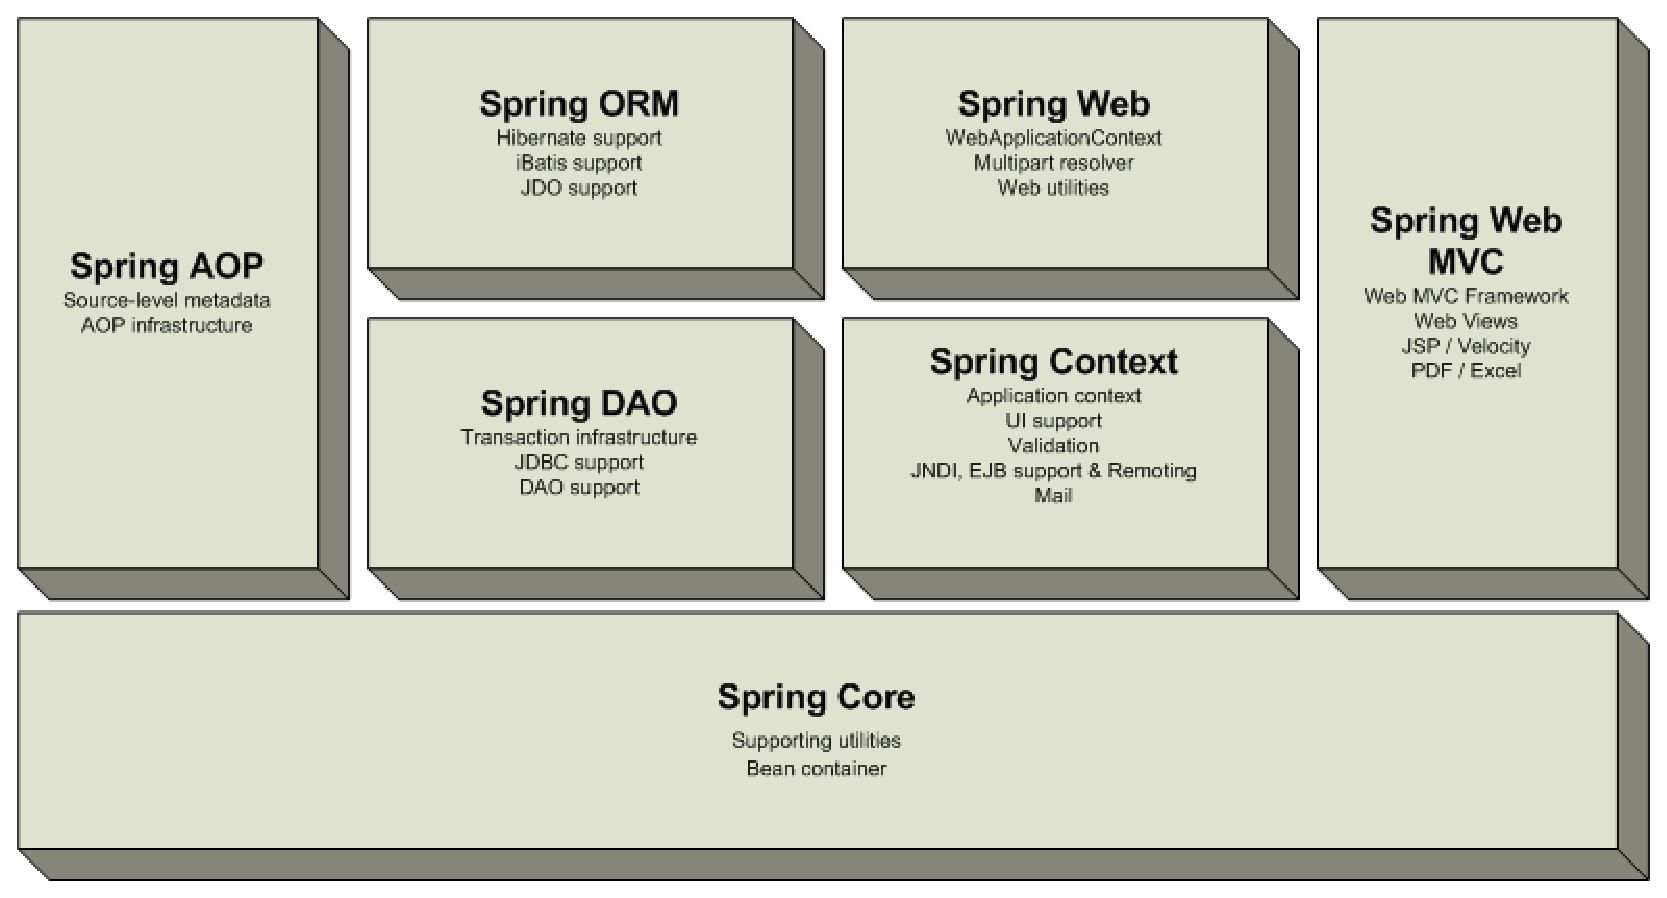
\includegraphics[width=15cm,height=7.9cm]{../images/finalreport/spring-overview.eps}
 \caption{Spring Framework Modules}
\end{figure}

ACE uses the following modules:
\begin{itemize}
 \item \emph{Core}
 \item \emph{Context}
 \item \emph{AOP}
\end{itemize}

The
\emph{Core} module provides the most fundamental part of \emph{Spring}, which
is the \emph{Dependency Injection} feature. With dependency injection,
not the bean itself grabs its dependencies with a service locator or
JNDI lookup but instead the dependencies are \emph{injected} by an
assembler into the bean. The assembler is called \emph{BeanFactory} in
Spring. This assembler also removes the need for programmatic singletons,
as Spring can ensure that the beans it manages are created only once. Further, 
it allows to remove the tedious \emph{wiring} of the whole application, which
is usually found in applications. For in depth information about
the concept of dependency injection visit 
\href{http://martinfowler.com/articles/injection.html}{http://martinfowler.com/\-articles/\-injection.html}.

The \emph{Context} module extends the \emph{Core} module by providing access
to internationalization features, application event propagation, and some
other additional features.

The Spring \emph{AOP} module provides an aspect-oriented programming 
implementation, which is compliant with interfaces defined by the 
\emph{AOP Alliance} 
(\href{http://aopalliance.sourceforge.net/}{http://aopalliance.\-.sourceforge\-.net/}). 
For instance it allows to transparently add method
interceptors to any object defined in the \emph{Spring} context. This allows
to implement so-called cross-cutting concerns, which tend to clutter the
core business logic. The Spring documentation contains a good introduction
about AOP concepts and it shows some very good usage examples.


\subsection{Simple Examples}

The \emph{BeanFactory} is one of the core interfaces in \emph{Spring}. 
Further, it is the actual \emph{container} which instantiates, configures, and 
manages a number of objects (factory service). 
These objects, called beans in Spring terminology, typcially have
dependencies to other objects also defined in the context. Bean factories
are represented by the \texttt{org.springframework.beans.factory.BeanFactory}
interface. There are several implementations of that interface. 
Usually most applications rely on the \emph{ApplicationContext} interface, which
extends the \texttt{BeanFactory} interface. 

Creating an application context is as simple as the following line of code:
\small{\begin{verbatim}
  ApplicationContext context = new ClassPathXmlApplicationContext("context.xml");
\end{verbatim}}

The passed in \emph{String} points to a resource on the classpath (in this 
case). The \texttt{context.xml} file is an XML file with the following
structure:

\small{\begin{verbatim}
<?xml version="1.0" encoding="UTF-8"?>
<!DOCTYPE beans PUBLIC "-//SPRING//DTD BEAN//EN" 
          "http://www.springframework.org/dtd/spring-beans.dtd">
<beans>
  
  <bean id="..." class="...">
    ...
  </bean>
  <bean id="..." class="...">
    ...
  </bean>

  ...
</beans>
\end{verbatim}}

The top-level \emph{beans} element contains an arbitrary number of \emph{bean}
sub-elements which represent objects managed by the \emph{Spring} container.
The \texttt{id} of a bean is a unique identifier of a managed bean in the 
\emph{Spring} container, which is used to reference that bean. 
The \texttt{class} argument specifies the class
of the object to be created. So the following creates a managed bean
with the id \texttt{exampleBean} of type \texttt{ExampleBeanClass}:

\small{\begin{verbatim}
  <bean id="exampleBean" class="ExampleBeanClass"/>  
\end{verbatim}}

\emph{Spring} can inject dependencies either through
constructor arguments or through Java Beans properties. Constructor arguments
are specified with the \texttt{constructor-arg} child element.

\small{\begin{verbatim}
  <bean id="exampleBean" class="ExampleBeanClass">
    <constructor-arg><ref bean="otherBean"/></constructor-arg>
  </bean>
  
  <bean id="otherBean" class="OtherBeanClass"/>
\end{verbatim}}

Properties of a bean are set through standard Java Beans property setter
methods.

\small{\begin{verbatim}
  <bean id="exampleBean" class="ExampleBeanClass">
    <property name="collaborator"><ref bean="otherBean"/></property>
  </bean>
  
  <bean id="otherBean" class="OtherBeanClass"/>
\end{verbatim}}

These are the basic features provided by \emph{Spring}. For more
details check the excellent documentation available at  
\href{http://static.springframework.org/spring/docs/1.2.x/reference/index.html}{http://static\-.springframework\-.org/\-spring/\-docs/\-1.2.x/\-reference/\-index.html}


\subsection{Advantages of Spring}

Using \emph{Spring} in an application has several advantages. We have a look
at some of these in the following sections.

\begin{itemize}
 \item encourages design to interfaces
 \item improved testability
 \item less tedious wiring code
\end{itemize}

\subsubsection{Design to Interfaces}
Spring encourages to split objects into an interface and an implementation.
This helps to clearly specify the methods that are needed to be exposed to
other objects. Further, interfaces provide the possibility to use completely
different implementations of the interface, which is also useful in testing.

\subsubsection{Improved Testability}
In a typical application, either the \emph{Service Locator} pattern 
or singletons are used to locate the dependencies. The use of the singleton
pattern makes it hard to unit test certain parts of the
application, because it is impossible to inject a custom object,

The availability of interfaces for most business objects as well as the
managed singletons of the \emph{Spring} container give us the possibility
to use \emph{Mock} objects as well as \emph{Stubs} to test our services
in isolation.

\subsubsection{Less Wiring Code}
In a mid-sized application there is a large amount of wiring code. The whole
object graph has to be set up. This wiring code is both tedious and
error-prone. \emph{Spring} removes the wiring process from the application
code into the framework. This might not seem a big deal, but after some time
using it, it becomes evident how much time can be saved.

It must be noted, that all the \emph{magic} done by \emph{Spring} could be
done by hand in the main method of the application. With \emph{Spring} all
this dirty hand-coded wiring of dependencies can be replaced by a 
declaration of all the dependencies in an XML file, which is easier to
analyze because of its declarative nature.


\section{Bonjour}
\label{chapter:frameworks.bonjour}
\subsection{Introduction}
Bonjour, formerly known as Rendezvous, enables automatic discovery of computers, devices, and services on IP networks. It uses industry standard IP protocols to allow devices to automatically discover each other without the need to enter IP addresses or configure DNS servers. It is a technology developed by Apple that is submitted to the IETF as part of an ongoing standards-creation process. The technology is more generally known as zero-conf networking. 

There are opensource Java libraries available that allow to use this technology in any Java application. The library needs a native library that is available for all major platforms. DNS service discovery is a way of using standard DNS programming interfaces, servers, and packet formats to browse the network for services. It is compatible with, but not dependent on, multicast DNS. Multicast DNS is a way of using familiar DNS programming interfaces, packet formats and operating semantics, in a small network where no conventional DNS server has been installed. 


\subsection{Usage}
The Bonjour API is small and provides a main class \texttt{DNSSD} to communicate with Bonjour and a set of listener interfaces to receive notifications and events, respectively. Figure \ref{fig:frameworks.dnssd.uml} shows the basic usage of the Bonjour API.

\begin{figure}[H]
 \centering
  \frame{
 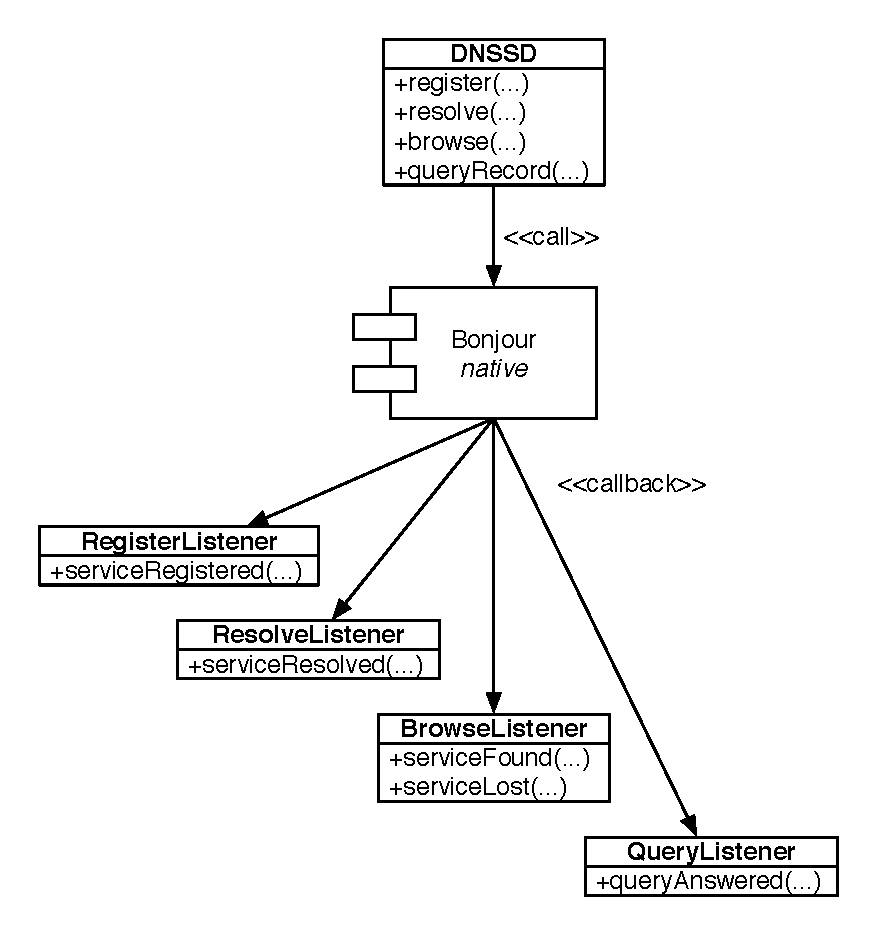
\includegraphics[width=5.62in,height=6.01in]{../images/finalreport/frameworks_dnssd_uml.eps}
 }
 \caption{\texttt{RequestHandler} Hierarchy}
 \label{fig:frameworks.dnssd.uml}
\end{figure}

Following the main functions of the Bonjour API are described. For further information see the references  section \ref{chapter:references}.

\subsubsection{Register a service}
To register a service, call \texttt{DNSS.register(...)} and pass an instance of \texttt{RegisterListener} which in turn is called back by Bonjour after the service was succesfully registered.

\subsubsection{Resolve a service}
In order to the get the target host name, the port number, and the TXT record of a service, the service must be resolved. To resolve a service, call \texttt{DNSSD.resolve(...)} and pass an instance of \texttt{ResolveListener} which in turn is called back by Bonjour when the service was successfully resolved. The TXT record can be used to store service specific metadata such as the version number or the id of the service instance.

\subsubsection{Browse for services}
The local area network can be browsed for specific service types. The service type to search for must be specified when calling \texttt{DNSSD.browse(...)} to start browsing. Besides, an instance of \texttt{BrowseListener} must be passed to call so that the application can be called back when new services of the specified type have been discovered or lost. When a new service is found, it must be resolved to get further service information depending on the application. 

\subsubsection{Query DNS record}
Each registered service can be queried for an arbitrary DNS record, e.g. its IP address or the contents of its TXT record. This is done by a call to \texttt{DNSSD.queryRecord(..)} which is passed an instance of \texttt{QueryListener} which is called back when a query record has been completed.

\subsection{mDNSResponder}
In order to use Bonjour, a small service for multicast DNS must be installed on the local host. mDNSResponder (also known as mdnsd on some systems) is a daemon to implement Multicast DNS and DNS Service Discovery (the discovery techniques used by Bonjour). mDNSResponder listens at UDP port 5353 for Multicast DNS Query packets. When it receives a query for which it knows an answer, mDNSResponder issues the appropriate Multicast DNS Reply packet. mDNSResponder also performs Multicast DNS Queries on behalf of client  processes, and maintains a cache of the replies (sometimes may arise caching problems in the sense that cached data (e.g. a former TXT record from user) is returned instead of the newest available data).


\section{BEEP Core}
\label{chapter:framework.beepcore}
\subsection{Introduction}
BEEP stands for Blocks Extensible Exchange Protocol. BEEP integrates the best practices for common, basic mechanisms that are needed when designing an application protocol over TCP. For example, it handles things like peer-to-peer, client/server, and server/client interactions.
The initial situation is that many Internet protocols reinvent a set of basic functions. The most common include: 

\begin{itemize}
\item Framing: separating each request from the next
\item Matching responses to requests 
\item Pipelining: permitting multiple outstanding requests 
\item Multiplexing: permitting multiple asynchronous requests 
\item Reporting errors 
\item Negotiating encryption 
\item Negotiating authentication 
\end{itemize}

BEEP specifies reusable tools for all these functions, instead of requiring the same decisions to be made over again for each new application. It provides a framework that integrates existing Internet standards for encryption and authentication and new standards for connection management. A networked application needs merely to supply the important part, the part that distinguishes it from other applications, as a BEEP profile. The mundane parts are the same for all protocols, and therefore can be coded as a library, freeing the application designer to focus on the interesting bits. The good thing about BEEP is that it solves common problems of most connection-oriented application protocols just once inside a framework. Further it is very efficient, requiring only a minimal overhead. BEEP is an inappropriate protocol if the protocol requires multicast or real-time support (for instance multicast video streaming). Figure \ref{fig:frameworks.beep.uml}

\begin{figure}[H]
 \centering
  \frame{
 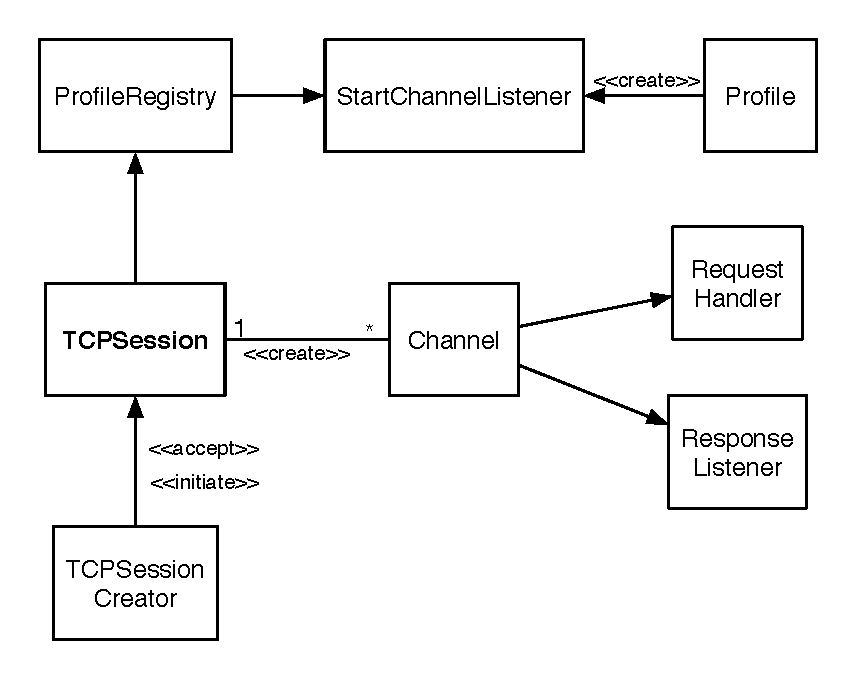
\includegraphics[width=5.49in,height=4.31in]{../images/finalreport/frameworks_beep_uml.eps}
 }
 \caption{Basic BEEP classes}
 \label{fig:frameworks.beep.uml}
\end{figure}



The basic code for the session listener looks as follows (executed in an separate thread):

\begin{verbatim}

public void run() {
     while (true) { 
          if (startup) {
               String profileURI = "http://myprofileuri.com/profiles/";
               Profile theProfile = new MyProfileImplementation();
               StartChannelListener listener = myprofile.init(theProfile, null);
               ProfileRegistry registry = new ProfileRegistry();
               registry.addStartChannelListener(profileURI, listener, null);
               startup = false;
          }
          //listens for new sessions
          TCPSessionCreator.listen(port, registry);
     }
}

\end{verbatim}

As the code example shows, an application must provide implementations for interfaces \texttt{Profile} and \texttt{StartChannelListener}. When the \texttt{TCPSessionCreator} accepted a new session, method \texttt{startChannel(...)} of \texttt{StartChannelListener} will be called so that the application can handle the channel appropriately (e.g. set the \texttt{RequestHandler} for the channel).

The basic code for the session initiator looks as follows:

\begin{verbatim}

public void createSession() {
     //create the same type of ProfileRegistry as the listener
     ProfileRegistry registry = createRegistry();
     TCPSession newSession = TCPSessionCreator.initiate(host, port, registry);
     //requests from the other peer are received via the RequestHandler
     RequestHandler handler = new MyRequestHandler();
     Channel channel = newSession.startChannel(profileURI, handler);
     ResponseListener listener = new MyReplyListener();
     //sends a mesage to the peer
     byte|[] message = createMessage();
     channel.sendMSG(message, listener);
     //the reply is received via the ResponseListener
}	
\end{verbatim}

As the code example shows, an application must provide implementations for interfaces \texttt{RequestHandler} and \texttt{ResponseListener}. Note that the exception handling was left out in the code examples for simplicity.


\subsection{Concepts}
BEEP is a peer-to-peer protocol in the sense that there is no notion of client or server. For convenience we�ll refer to the peer that starts a connection as the \emph{initiator}, and the peer accepting the connection as the \emph{listener}. When a connection is established between the two, a BEEP session is created.

\subsubsection{Profiles}
After the establishment of a session, the initiator asks to start a channel for the particular profile or set of profiles it whishes to use. If the listener supports the profile(s), the channel will be created. Profiles themselves take one of two forms: those for initial tuning and those for data exchange. Tuning profiles, set up at the start of communication, affect the rest of the session in some way. For instance, requesting the TLS profile ensures that channels are encrypted using Transport Layer Security. Other tuning profiles perform steps such as authentication. Data exchange profiles set expectations between the two peers as to what sort of exchanges will be allowed in a channel. A profile is identified by a URI. 

\subsubsection{Channels}
All communication in a session happens within one or more channels. The peers require only one IP connection, which is then multiplexed to create channels. The nature of communication possible within that channel is determined by the profiles it supports (each channel may have one or more). The first channel, channel 0, has a special purpose. It supports the BEEP management profile, which is used to negotiate the setup of further channels. The supported profiles determine the precise interaction between the peers in a particular channel. Defining a protocol in BEEP comes down to the definition of profiles. 

\subsubsection{Data types}
BEEP puts no limits on the kind of data a channel can carry. It uses the MIME standard to support payloads of arbitrary type. 



\section{Glazed Lists}
\label{appendix_frameworks_glazedlists}
\subsection{Introduction}
\textit{Glazed Lists} (see \href{http://www.publicobject.com/glazedlists/}{http://www.publicobject.com/glazedlists/}) is a framework written in \textit{Java} that makes building applications based on tabular data very easy to produce. \textit{Glazed Lists} contains the following features that are interessting for our application development:
\begin{itemize}
\item EventList
\item SortedList
\item FilterList
\end{itemize}
The following sections explaining the basics of these features, why they are interessting for our application development and some simple code fragments of their usage.

\subsection{EventList}
\label{frameworks_glazed_eventlist}
An \textit{EventList} is an interface that extends \texttt{java.util.List}. It represents an observable list which makes it possible to add and remove \textit{List\-Event\-Listeners}. Further, there is a possibility to get a read/write lock to control concurrency access to the list.

% TODO: make more precise
An \textit{Observable\-Element\-List} is a list that fires update events whenever elements are modified in place. Changes to list elements are detected by registering an appropriate listener on every list element. \textit{List\-Event\-Listeners} are registered as elements are added to this list and unregistered as elements are removed from this list. A \textit{Observable\-Element\-List.Connector} needs to be specified in the constructor which contains the necessary logic for registering and unregistering an appropriate listener for detecting modifications to list elements.

The following example shows the use of a \textit{Basic\-Event\-List} (the most basic implementation of the \textit{Event\-List}) for a GUI component. The class \textit{User} is a very simple class that has a username property. It uses a \textit{Property\-Change\-Support} instance to manage and notify all registered \textit{Property\-Change\-Listeners} whenever a new name has been set through the method \texttt{setName(...)}.

\begin{verbatim}
  public class User {
    private String name;
    private PropertyChangeSupport propertyChangeSupport;

    public User(String name) {
      this.name = name;
      propertyChangeSupport = new PropertyChangeSupport(this);
    }
    
    public void addPropertyChangeListener(PropertyChangeListener listener) {
      propertyChangeSupport.addPropertyChangeListener(listener);
    }

    public void removePropertyChangeListener(PropertyChangeListener listener) {
      propertyChangeSupport.removePropertyChangeListener(listener);
    }
    
    public String getName() { return name; }
    
    public void setName(String name) {
      String oldName = this.name;
      this.name = name;
      support.firePropertyChange("name", oldName, name);
    }
  }
\end{verbatim}

Assume a simple GUI component that displays the list of users in a \textit{JList}. By wrapping an \textit{Observable\-Element\-List} and an \textit{Event\-List\-Model} around the list of users, the \textit{JList} diplaying the users will be automatically notified whenever a user changes his name and will repaint the element with the new username.

\begin{verbatim}
  // create a list of users
  EventList users = new BasicEventList();
  users.add(new User("Mark Bigler"));
  users.add(new User("Simon Raess"));
  users.add(new User("Lukas Zbinden"));

  // create the observable list
  EventList observableUserList = new ObservableElementList(users,
    GlazedLists.beanConnector(User.class)
  
  // create list & model
  JList userList = new JList(new EventListModel(observableUserList));
\end{verbatim}
 

\subsection{SortedList}
A \textit{Sorted\-List} is an \textit{Event\-List} that sorts another \textit{Event\-List}. The sorting strategy is specified with a \textit{Comparator}. If no \textit{Comparator} is specified, all of the elements of the source \textit{Event\-List} must implement \textit{Comparable}. The following example adds the \textit{Comparable} interface to the user class from the example in section \ref{frameworks_glazed_eventlist} and creates a \textit{Sorted\-List} out of the user list.

\begin{verbatim}
  public class User implements Comparable {
    // property change support, getter and setter methods not shown here
    
    // implements the compareTo method
    public int compareTo(Object o) {
      return -((User)o).getName().compareTo(name);
    }
  }
\end{verbatim}

This addition makes it possible to compare and sort objects of type {User}. A \textit{Sorted\-List} is now wrapped around the list of users and the \textit{JList} will display the users sorted by name (as specified in the \texttt{compareTo(...)}). Note that wrapping an \textit{Event\-List} with a \texttt{Sorted\-List} does not change the order of elements in the source list.

\begin{verbatim}
  // create list & observable list not shown here
  
  // create the sorted list
  SortedList sortedUserList = new SortedList(observableUserList);

  // create list & model
  JList userList = new JList(new EventListModel(sortedUserList));
\end{verbatim}


\subsection{FilterList}
The \textit{Filter\-List} filters another \textit{Event\-List}. It is an \textit{Event\-List} that shows a subset of the elements of the source list. This subset is composed of all elements of the source \textit{Event\-List} that match the filter.

Filtering can either be static or dynamic. \textbf{Static filtering} can be used for example to filter out  elements with a special type. Assume the class \textit{User} from the example in section \ref{frameworks_glazed_eventlist} has in addition the age of the user. Its is a simple \textit{int} with the corresponding setter and getter methods. For example, use the following code to filter out and display only the user older than 20 years:
\begin{verbatim}
  // create a matcher for matching user objects including the age
  Matcher ageMatcher = new Matcher() {
    public boolean matches(Object item) {
      User uItem = (User)item;
      return (uItem.getAge() > 20);
    }
  };

  // create the filtered list
  FilterList userFilterList = new FilterList(observableUserList, ageMatcher);

  // create list & model
  JList userList = new JList(new EventListModel(userFilterList));
\end{verbatim}

\textbf{Dynamic filtering} can be used for example if the list of users should be filtered by user names and the filter can change. The following example uses a \textit{JTextField} containing the filter string. The filtered user list contains only the users matching the enetered text.

\begin{verbatim}
  // create the filter field and the text filterator
  JTextField nameFilterField = new JTextField();

  TextFilterator nameFilterator = new TextFilterator() {
    public void getFilterStrings(List baseList, Object element) {
      User utem = (User)element;
      baseList.add(item.getName));
    }
  };

  // create the needed matcher editor
  MatcherEditor nameMatcherEditor =
    new TextComponentMatcherEditor(nameFilterField, nameFilterator);
  
  // create dynamic filter list
  FilterList userFilterList = new FilterList(observableUserList, nameMatcherEditor);

  // create list & model
  JList userList = new JList(new EventListModel(userFilterList));
\end{verbatim}

\subsection{Summary}
Using \textit{Glazed Lists} for GUI programming (or even other applications using data tables) speeds up the implementation process because you dont have to care about simple things like sorting, filtering or updating list elements. It is worth to spend some time to learn the basics of using \textit{EventLists}.

